
%%%%%%%%%%%%%%%%%%%%%%% file typeinst.tex %%%%%%%%%%%%%%%%%%%%%%%%%
%
% This is the LaTeX source for the instructions to authors using
% the LaTeX document class 'llncs.cls' for contributions to
% the Lecture Notes in Computer Sciences series.
% http://www.springer.com/lncs       Springer Heidelberg 2006/05/04
%
% It may be used as a template for your own input - copy it
% to a new file with a new name and use it as the basis
% for your article.
%
% NB: the document class 'llncs' has its own and detailed documentation, see
% ftp://ftp.springer.de/data/pubftp/pub/tex/latex/llncs/latex2e/llncsdoc.pdf
%
%%%%%%%%%%%%%%%%%%%%%%%%%%%%%%%%%%%%%%%%%%%%%%%%%%%%%%%%%%%%%%%%%%%


\documentclass[runningheads,a4paper]{llncs}

\usepackage{amssymb,amsmath}
\setcounter{tocdepth}{3}
\usepackage{graphicx}
\DeclareMathOperator*{\argmin}{arg\,min}
\usepackage{subfigure, caption}

\usepackage{url}
%\urldef{\mailsa}\path{a.churchill,ssgd,c.t.fernando}@qmul.ac.uk
\newcommand{\keywords}[1]{\par\addvspace\baselineskip
\noindent\keywordname\enspace\ignorespaces#1}

\begin{document}

\mainmatter  % start of an individual contribution

% first the title is needed
\title{An Estimation of Distribution-like Algorithm based on a Denoising Autoencoder}

% a short form should be given in case it is too long for the running head
\titlerunning{An EDA-like Algorithm based on a Denoising Autoencoder}

% the name(s) of the author(s) follow(s) next
%
% NB: Chinese authors should write their first names(s) in front of
% their surnames. This ensures that the names appear correctly in
% the running heads and the author index.
%
\author{Alex%
%
\and Sid\and Chrisantha}
%
\authorrunning{Alex, Sid and Chrisantha}
% (feature abused for this document to repeat the title also on left hand pages)

% the affiliations are given next; don't give your e-mail address
% unless you accept that it will be published
\institute{School of Electronic Engineering and Computer Science\\Queen Mary, University of London\\
{\{a.churchill,ssgd,c.t.fernando\}}@qmul.ac.uk}

%
% NB: a more complex sample for affiliations and the mapping to the
% corresponding authors can be found in the file "llncs.dem"
% (search for the string "\mainmatter" where a contribution starts).
% "llncs.dem" accompanies the document class "llncs.cls".
%

\toctitle{Lecture Notes in Computer Science}
\tocauthor{Authors' Instructions}
\maketitle


\begin{abstract}
In this paper we present a novel neural-based optimisation algorithm. The algorithm follows the traditional generate-update methodology of Estimation of Distribution algorithms, using a denoising autoencoder to learn the structure of promising solutions within its hidden layer, with the output neurons defining a probability distribution that is sampled from to produce new solutions. The algorithm is shown to outperform a canonical Genetic Algorithm on several combinatorial problems, including the multi dimensional 0/1 knapsack problem, MAXSAT and the Hierarchical If and Only If. Analysis shows that the neural network is able to learn interesting structural features of the search space, while the sampling method employed supports continued exploration, enabling optimal solutions to be found on NP-hard problems.
\end{abstract}


\section{Introduction}

Estimation of Distribution Algorithms (EDAs) are a growing field in Evolutionary Computation, which attempt to build a statistical model of sections of a search space in order to uncover underlying structure and guide search in an efficient manner \cite{pelikan2006scalable}. At the heart of an EDA lies a model-building algorithm. Examples include Bayesian Networks \cite{hboa}, Markov Networks \cite{ref} and K-Means clustering \cite{ref}. In this paper we introduce a novel neural-based method for modelling, a denoising autoencoder. An auto encoder is a feed forward neural network, consisting of at least one hidden layer, which is trained to reproduce its inputs from its outputs. Over the course of training the hidden layer learns a representation of the data, which has been applied to reconstructing missing data \cite{ref} and dimensionality reduction \cite{ref} in Machine Learning applications. The algorithm introduced in this paper trains a single autoencoder with promising solutions from a population, from which structure of the search space is learnt by the representation in the hidden layer. This differs from traditional EDAs such as PBIL \cite{ref } or ECGA \cite{ref} as an explicit statistical model is not produced. However, the learnt structure can be leveraged to produce new solutions by inputting an existing or randomly generated solution into the network and sampling from the output neurons using a binomial distribution. Results presented in Section 6 show that the autoencoder method is able to outperform a canonical Genetic Algorithm on a range of combinatorial and hierarchical problems.

\section{Background}

EDAs (also known as Probabilistic-Model-Building Genetic Algorithms) are population based optimisers, that typically replace genetic operators with a statistical model. The rationale behind the model building and related linkage learning approach is that dependencies between variables can be captured and preserved, which can be easily lost in standard Evolutionary Search, and new solutions generated around promising structures. Early work on EDAs concentrated on methods that explicitly modelled the probabilities of independent alleles occurring in a population of genotypes. These include the compact Genetic Algorithm \cite{cha}, PBIL \cite{phil} and Univariate Marginal Probability methods\cite{uvmp}. Improved success was found by modelling multivariate dependencies using clustering algorithms (ECGA) \cite{ecga}, Bayesian Networks \cite{hboa}, Markov Networks \cite{mccall} and tree structures \cite{ltga}, among others. The use of the autoencoder model in this paper is motivated by its potential to learn high-dimensional dependencies in data, while still maintaining a low computational cost in terms of training time. Recently there has been interest in neural-based methods in an EDA context for multi-objective optimisation. A Growing Neural Gas (GNG) was used as a model in \cite{moneda}, employing a competitive Hebbian learning rule to cluster data without having to pre specify the number of groups. A shallow Restricted Boltzmann Machine (RBM) was used to model high dimensional data in \cite{singapore}. An autoencoder is another neural-based method for unsupervised learning of features that has potential to model solution structure and has hitherto not been applied to combinatorial or continuous optimisation.

A second motivation for this approach is to investigate methods in which Evolutionary Algorithms can be implemented in neural structures. The {\em{Neural Replicator Hypothesis}} \cite{ref} proposes that evolutionary processes could operate in the brain at ontogenetic timescales. In \cite{fernando2010neuronal} a network of spiking neurons combined with Hebbian learning, which enabled linkages to be found between features, was applied to combinatorial problems and solved the 128-bit HIFF problem.

\section{Methods}

\subsection{Denoising Autoencoder}

A standard autoencoder consists of an encoder and a decoder. The encoder performs an affine transformation followed by an element-wise non-linear operation. The mapping performed by the encoder is deterministic and can be described as: $$h_{\theta}(\mathbf{x}) = f(\mathbf{Wx + b})$$ The non-linear activation function $f$ can be any one of the standard non-linearities used in artificial neural networks (sigmoid,tanh). The encoder parameters are $\mathbf{\theta = \left\{ W,b \right\}}$. 

The decoder is also a deterministic function and operates on the encoded input $h_{\theta}(x)$ to produce the reconstructed input: $$ r_{\theta'}(\mathbf{h}) = g(\mathbf{W'h + b'})$$ 
The decoder parameters are $\mathbf{\theta' = \left\{ W',b' \right\}}$. The output non-linearity, $h$ can vary depending on the whether the input data is binary or continuous. The outputs of the decoder are generally not considered as exact reconstructions, but parameters for some distribution $p(X|Z=\mathbf{z})$. 

\subsection{Training}

For combinatorial problems, the inputs $\mathbf{x} \in \left\{ 0,1 \right\}^d$. The decoder must produce a binary output, therefore reconstructed outputs $z$ are considered to be parameters for the distribution  $X|\mathbf{z} \sim \mathcal{B(\mathbf{z}})$ where $\mathcal{B}$ is the bernouilli distribution. The autoencoder is trained by minimizing the loss function w.r.t to the model parameters using stochastic gradient descent:
$$ \theta^{*},\theta'^{*} = \argmin_{\theta,\theta'}{\frac{1}{n}}\sum_{i=1}^{n}\mathcal{L}(\mathbf {x^{(i)},z^{(i)}})$$
For binary inputs, we use the cross-entropy loss function. The cross-entropy loss function can be viewed as the negative log-likelihood of the training vector $\mathbf{x}$ given the parameters for the bernouilli distribution $\mathbf{z}$. The loss function $\mathcal{L}$ is defined as:
$$ \mathbf{\mathcal{L}(x,z) = -\sum_{j}[x_{j} \log z_{j} + (1 - x_{j})\log {(1-z_{j})}]}$$ 
Empirical evidence suggests that training autoencoders by only minimizing reconstruction loss might not be enough to learn useful representations in the hidden layer. An autoencoder with enough capacity can easily learn the identity function, thus reconstructing the input perfectly each time, which is not very useful. In order to force the network to learn interesting transformations, an information bottleneck must be imposed during training. A common approach is to set the number of hidden units to be smaller than the dimensionality of the data. This ensures that the network must discover structure in the inputs in order to reconstruct with high accuracy. Tying the weights of the encoder and decoder networks to be the same is another method used to guide training. Apart from these techniques, the standard regularisation techniques like L1 and L2 weight \cite{bishop1995neural} decay are also employed while training autoencoders. 

\subsection{Denoising Autoencoders}

With the revival of interest in neural nets and deep neural architectures, several new variants of autoencoders have been proposed which differ in the kind of regularisation used during training \cite{vincent2010stacked,rifai2011contractive}. The denoising autoencoder is a particularly interesting variant of the classical autoencoder that tries to reconstruct a \textit{clean} version of a noisy example, thus \textit{denoising} noisy inputs. 

The input $\mathbf x$ is first corrupted using a stochastic corruption process $\mathbf{\tilde x = q(\tilde x|x)}$. The corrupted input is then mapped to a hidden representation $\mathbf h$ by the encoder. Finally, the decoder tries to reconstruct the uncorrupted input $\mathbf x$ from $\mathbf h$. The denoising autoencoder is trained by minimizing the cross-entropy loss on the training set using stochastic gradient descent. The functioning of the denoising autoencoder can be interpreted in two ways. One view is that forcing the network to reconstruct clean inputs from corrupted inputs acts as a regulariser. It ensures that training must converge to networks that learn transformations more complex than the identity function. Denoising autoencoders also have a geometric interpretation \cite{vincent2010stacked}. A denoising autoencoder learns the distribution $p(X|\tilde X)$. This distribution maps noisy inputs to clean examples seen in the training set. Therefore the denoising encoder maps points from regions of low probability to regions of higher probability. These points with higher probability mass are said to form a low dimensional manifold according to the manifold assumption \cite{chapelle2006semi}. Under this interpretation, denoising autoencoders can be used for learning manifolds in input space.

\subsection{Autoencoders and Genetic Algorithms}
EDAs try to improve GA convergence by building a distribution of the most promising solutions at each generation and sampling a new population of solutions from this distribution. Therefore the two main requirements for building an effective EDA are efficient distribution estimation from training examples and efficient sampling from the learned distribution[citation]. In this work we propose an alternative approach to model building and sampling using denoising autoencoders. 

Using the dAE to model conditional distributions has the advantage that the network is trained with standard backpropagation, which is deterministic and does not involved any sampling. This leads to quick and efficient training of models at each generation. dAEs are also advantageous because the output distribution of the network given a reconstruction $ \mathbf z$ is  $X|\mathbf{z} \sim \mathcal{B(\mathbf{z}})$. Therefore sampling new solutions involves sampling from a bernoulli distribution which is much simpler compared to sampling from more complex distributions [examples,citations]. 

The proposed algorithm differs from a standard EDA in the fact that we model conditional distributions $p(X|\tilde X)$ instead of distributions of the input $p(X)$. Although denoising was introduced as a regulariser for learning better networks \cite{vincent2010stacked}, we find it particularly well suited for modelling in a GA. It forces bad samples towards better samples from the distribution, by means of the conditional probability distribution which maps inputs that are far from the `good' solutions towards them.

Another challenging problem associated with EDAs is the problem of maintaining a good variance in the newly sampled population, so that the GA can explore the space effectively. The problem of EDAs converging to a few points has been observed in several cases [citations]. With the conditional distribution, we can control the variance in the output, by choosing inputs that are reasonably diverse. This ensures that the new population has enough variance to perform search effectively. 



\subsection{Optimisation Algorithm}

The pipeline of DAGA is similar to other EDAs and incorporates techniques from HBOA \cite{hboa}. A population of solutions is maintained, \(P_t\), updated at each iteration, \(t\). An initial population of solutions, \(P_0\), is drawn from a uniform distribution. These solutions are evaluated and the fittest unique x\% are selected (i.e. truncation selection) to be in the training set, \(\hat{P_t}\). The Denoising Autoencoder, \(D_t\), is then trained with \(\hat{P_t}\) for \(e\) epochs. Following training, a new set of solutions, \(S_t\), is selected from \(P\) using tournament selection (with replacement). Each member of \(S_t\) is inputted to \(D_t\), and the output vector, \(y\), is sampled from using a binomial distribution, to produce a new solution. This solution is included in \(P_{t+1}\) if it is better than its closest neighbour according to Restricted Tournament Selection (RTR) \cite{hboa}. Pseudocode for DAGA is presented in Algorithm 1.

\section{Experiments}
\label{sec:experiments}
Experiments intro blurb.

\subsection{Multi-dimensional Knapsack Problem}
Here we wish to choose of subset of \(N\) items to maximise the total value of items, \(z\), while satisfying \(m\) constraints. We wish to maximise:
\vspace{2mm}\\
\(z = \sum_{j=1}^{N} v_jx_j\), subject to \(\sum_{j=1}^{N} w_{ij}x_i \leq c_i, i = 1, ..., m\)
\vspace{2mm}\\
\(x_i \in \{0,1\}, j = 1, ..., N\).
\vspace{2mm}\\
In the results below, two problems are tackled. The first is the Weing8 instance \cite{ref}, which has 105 items and two constraints (optimal solution is 602,319), and the second is a randomly generated instance with 500 items and one constraint (optimal solution is 104,000). Both instances are available in the supplementary material. If any constraint is violated, the total value of chosen items is multiplied by \(-1\).

\subsection{Hierarchical If and only If}

\subsection{Royal Road}
The Royal Road function as defined by Mitchell et al. \cite{mitchell}, divides a bit string into a number of  equally sized, non-overlapping partitions. If all of the bits in the partition are correct (e.g. all 1s), then the partition's fitness contribution is added to the overall fitness. The existence of these ``Building blocks" was meant to act as a ``royal road" for GAs compared to hill-climbers but bad alleles hitchhiking to good partial solutions slows down convergence speed. The problem is defined as,
\\
\[
s(i) = sum of bits...
\]
 
\subsection{MAXSAT}

\section{Results}
\begin{figure}[t!]
\centering
\subfigure[]{
\makebox[.47\textwidth]{
    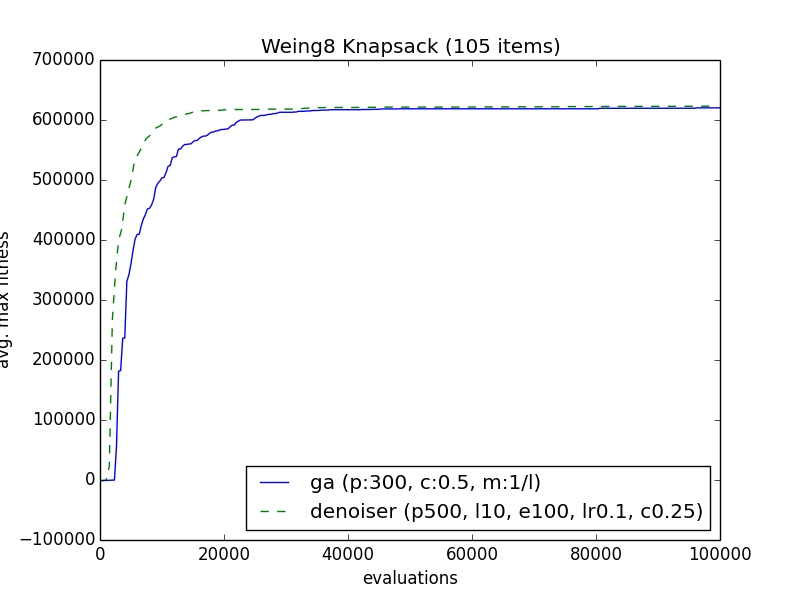
\includegraphics[scale=0.35]{images/105_knapsacks.png}
    \label{fig:subfig1}
    }
}
\subfigure[]{
\makebox[.47\textwidth]{
    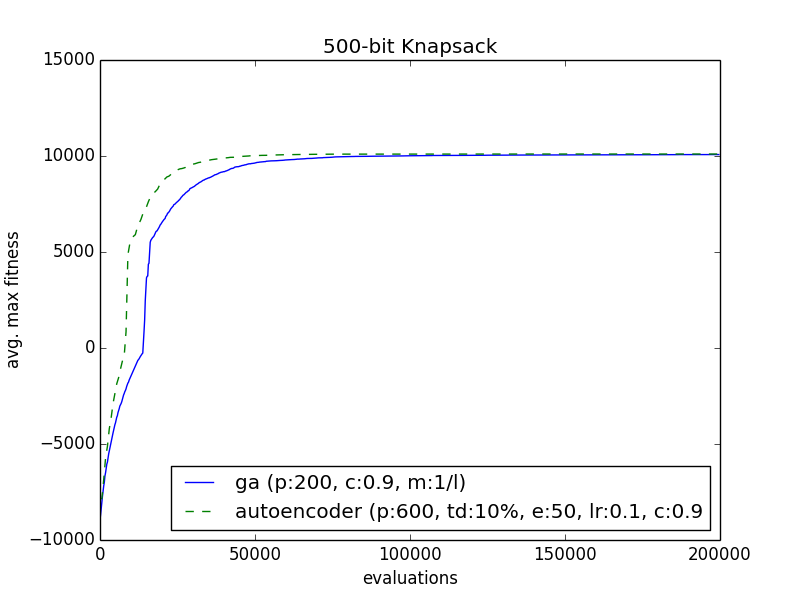
\includegraphics[scale=0.35]{images/knapsack_500_results.png}
    \label{fig:subfig2}
    }
}
\subfigure[]{
\makebox[.47\textwidth]{
    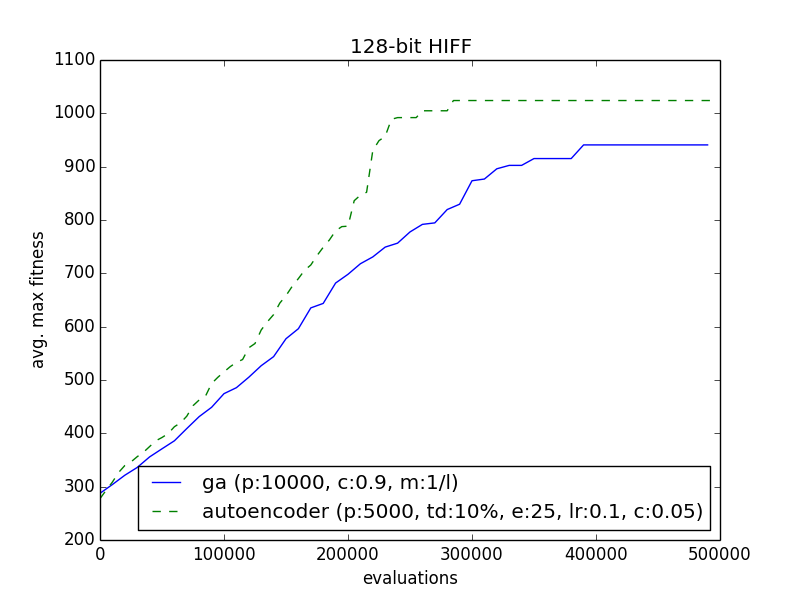
\includegraphics[scale=0.35]{images/128_hiff_results.png}
    \label{fig:subfig3}
    }
}
\subfigure[]{
\makebox[.47\textwidth]{
    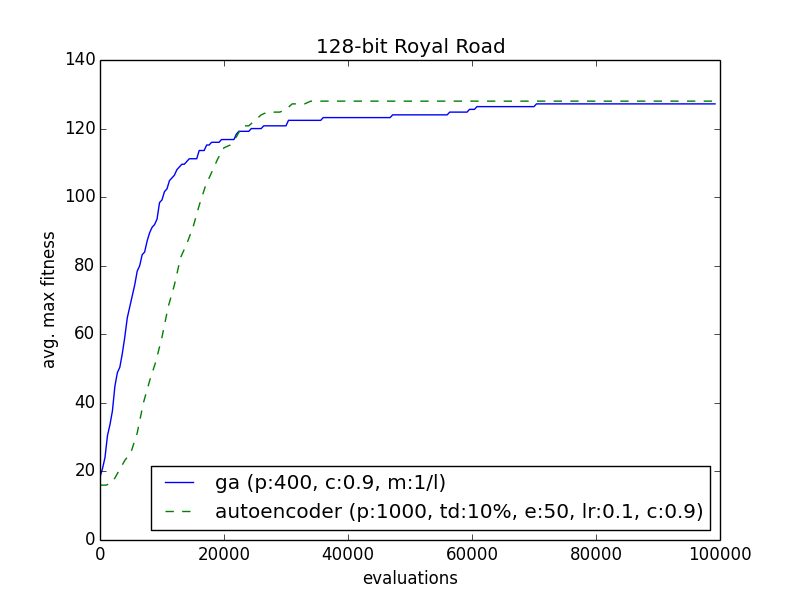
\includegraphics[scale=0.35]{images/royal_road_128_results.png}
    \label{fig:subfig3}
    }
}

\caption[Optional caption for list of figures]{Plots showing the mean fitness of the best solution in the population over time, averaged over 10 trials.}
\label{figure:experiment_subplots}
\end{figure}

DAGA is compared to a canonical generational Genetic Algorithm (GA) on the problems described in Section~\ref{sec:experiments}. The GA employs tournament selection to select parents, two point crossover for recombination (with probability \(p_c\)) and a probability, \(p_m\), of a bit flip mutation at each allele. The GA is implemented in the DEAP framework \cite{deap}, while DAGA is implemented in Python, using Theano for the \(dA\). Programming code is available in the online supplementary material.  For each experiment a large parameter sweep was performed on both DAGA and the GA and the best configurations were chosen for comparison. Figure~\ref{figure:experiment_subplots} presents graphs showing the mean fitness (averaged over ten trials) of the best solution in the population at each iteration for the two algorithms on the 5 problems. Details of the best solutions found are given in table~\ref{}.

From Figure~\ref{figure:experiment_subplots}  we can immediately see that DAGA finds significantly better solutions than the GA or optimal solutions significantly faster than the GA. On three of the five experiments (both knapsacks and MAXSAT), DAGA finds significantly better results than the GA is able to, given the evaluation limits. On the Weing8 instance DAGA reaches the optimum solution 8 out of 10 attempts, and on the 500-item instance 7 out of 10 attempts. On the MAXSAT instance, DAGA also reaches the optimum 70\% of the time. On all three of these problems the GA is unable to locate the optimal solution a single time, within the evaluation limits. On the HIFF, DAGA locates the optimal solution every time, while the GA locates it on only half of the trials. On the Royal Road, DAGA again locates the optimum on every trial, while the GA finds it 9 out of 10. These results show that DAGA is able to find higher quality solutions and more consistently locate the optimum compared to the GA, across a wide range of problems.



% Talk about speed and significance at different running times
% Talk about how a solution "evolves".
% Talk about sensitivity on corruption.

\section{Discussion}
% HyperPothesis: When the input features are independent then high corruption helps because you don't care about information in the input as much, and you're forcing solutions to have a similar structure (the output structure is not dependant on the input structure because independent. On structured problems like the HIFF there is a lot of information in the inputs, so distorting this discards the information that might be useful.)
\section{Conclusion}

\subsubsection*{Acknowledgments.} The work is funded by the FQEB Templeton grant ``Bayes and Darwin", and the FP-7 FET OPEN Grant INSIGHT.

\bibliographystyle{splncs}
\bibliography{autoencoder_ppsn}

\end{document}
